\section{Auswertung der Erfüllung der Kriterien nach ISO 9241-110}
Einleitungstext ...\\
Die Erfüllung der Kriterien wird bewertet mithilfe einer Mischung beider Validierungsverfahren bewertet\\

\noindent
ISO-Kriterien:
\begin{itemize}
    \item Aufgabenangemessenheit (aa) - 1,2,8 + Usability-Test wenn Aufgaben durchführbar
    \item Selbstbeschreibungsfähigkeit (sb) - 10
    \item Erwartungskonformität (ek) - 4,5\\
    -> es gab Feedback nach Usability-Test
    \item Erlernbarkeit (if) - 6,7,9 + Usability-Test bei ähnlichen Zeitergebnissen
    \item Steuerbarkeit (SK) - 3
    \item Robustheit gegen Benutzungsfehler (ft)\\
    -> in diesem Use-case nicht benötigt (keine Eingaben möglich)\\
    -> wird durch Usability-Test überprüft
    \item Benutzerbindung (ik) - gehört zur User-Experience und ist kein Bestandteil dieser Arbeit
\end{itemize}

\subsection*{ISO-Kriterium Aufgabenangemessenheit}
\begin{figure}[H]
    \centering
    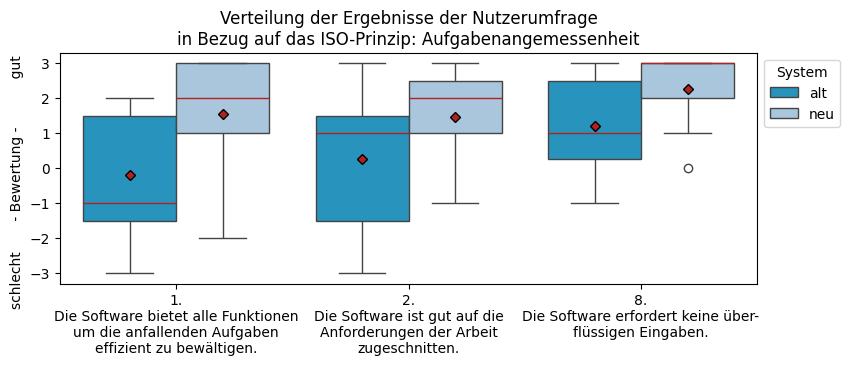
\includegraphics[width=1\linewidth]{Diagramme/pruemper_aa.png}
    \caption{Auswertung der Fragen bzgl. Gestaltungskriterium Aufgabenangemessenheit nach ISO 9241-110 (Ausschnitt aus \autoref{fig:pruemper_all})}
    \label{fig:pruemper_Aufgabenangemessenheit}
\end{figure}

\noindent
t-Test von Fragen 1 \& 8 sind signifikant (<0.5)\\
wenn bei 2 die beiden Ausreißer weggenommen werden, die andersrum bewertet haben, dann wird der Unterschied auch signifikant (s. \autoref{fig:hist_prümper_all})\\
Boxplot: \autoref{fig:pruemper_Aufgabenangemessenheit}
\subsection*{ISO-Kriterium Steuerbarkeit}

\begin{figure}[H]
    \centering
    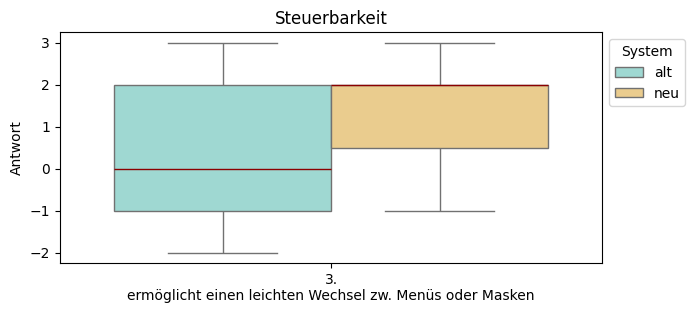
\includegraphics[width=1\linewidth]{Diagramme/pruemper_sk.png}
    \caption{Auswertung der Fragen bzgl. Gestaltungskriterium Steuerbarkeit nach ISO 9241-110 (Ausschnitt aus \autoref{fig:pruemper_all})}
    \label{fig:pruemper_Steuerbarkeit}
\end{figure}


\subsection*{ISO-Kriterium Erwartungskonformität}

\begin{figure}[H]
    \centering
    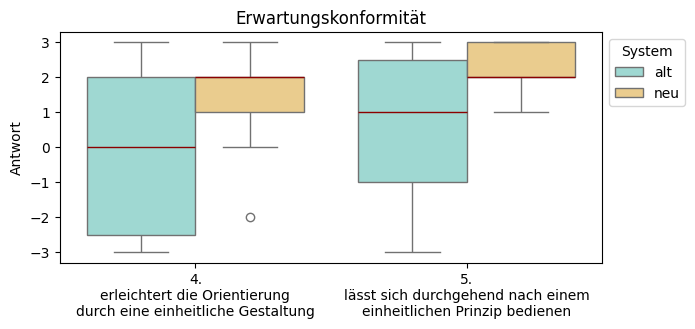
\includegraphics[width=1\linewidth]{Diagramme/pruemper_ek.png}
    \caption{Auswertung der Fragen bzgl. Gestaltungskriterium Erwartungskonformität nach ISO 9241-110 (Ausschnitt aus \autoref{fig:pruemper_all})}
    \label{fig:pruemper_Erwartungskonformität}
\end{figure}

\noindent
t-Test von Fragen 1 \& 8 sind signifikant (<0.5)\\
Boxplot: %\autoref{fig:pruemper_Erwartungskonformität}

\subsection*{ISO-Kriterium Erlernbarkeit}
\begin{figure}[H]
    \centering
    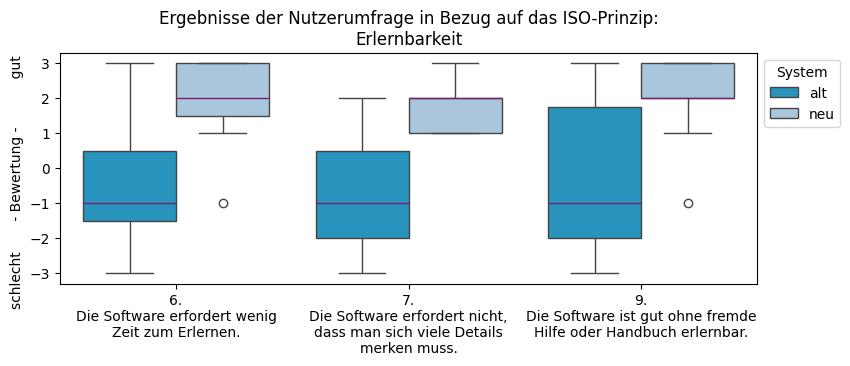
\includegraphics[width=1\linewidth]{Diagramme/pruemper_if.png}
    \caption{Auswertung der Fragen bzgl. Gestaltungskriterium Erlernbarkeit nach ISO 9241-110 (Ausschnitt aus \autoref{fig:pruemper_all})}
    \label{fig:pruemper_Erlernbarkeit}
\end{figure}

\noindent
t-Test von Fragen 6, 7 \& 9 sind signifikant (<0.5) - s. \autoref{tab:Nutzerbefragung:Differenz+ttest}\\
Boxplot: \autoref{fig:pruemper_Erlernbarkeit}
\subsection{ISO-Kriterium Selbstbeschreibungsfähigkeit}
\begin{figure}[H]
    \centering
    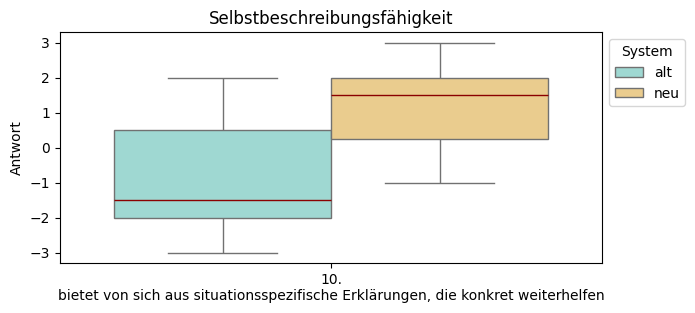
\includegraphics[width=1\linewidth]{Diagramme/pruemper_sb.png}
    \caption{Auswertung der Fragen bzgl. Gestaltungskriterium Selbstbeschreibungsfähigkeit nach ISO 9241-110 (Ausschnitt aus \autoref{fig:pruemper_all})}
    \label{fig:pruemper_Selbstbeschreibungsfähigkeit}
\end{figure}

\noindent
t-Test von Fragen 1 \& 8 sind signifikant (<0.5)\\
Boxplot: \autoref{fig:pruemper_Selbstbeschreibungsfähigkeit}

\subsection*{ISO-Kriterium Robustheit gegen Benutzungsfehler}
-	in diesem Use-case nicht benötigt (es gibt keine Fehler-Anzeigen)
-	wird durch Usability-Test überprüft -> Fehlerquote\\
-> ABER: auf Fehlergründe eingehen

\subsection{ISO-Kriterium Benutzerbindung}
-> Abgrenzung von UX(!)

% Zusammenfassung?
